\documentclass{article} % say
\usepackage{tikz}
\usetikzlibrary{calc,fit,positioning,arrows}


\begin{document}
\tikzset{pop1/.style={blue!40},pop2/.style={red!40}}
%\tikzstyle{pop2 place}= [place,draw=red,fill=red!40]

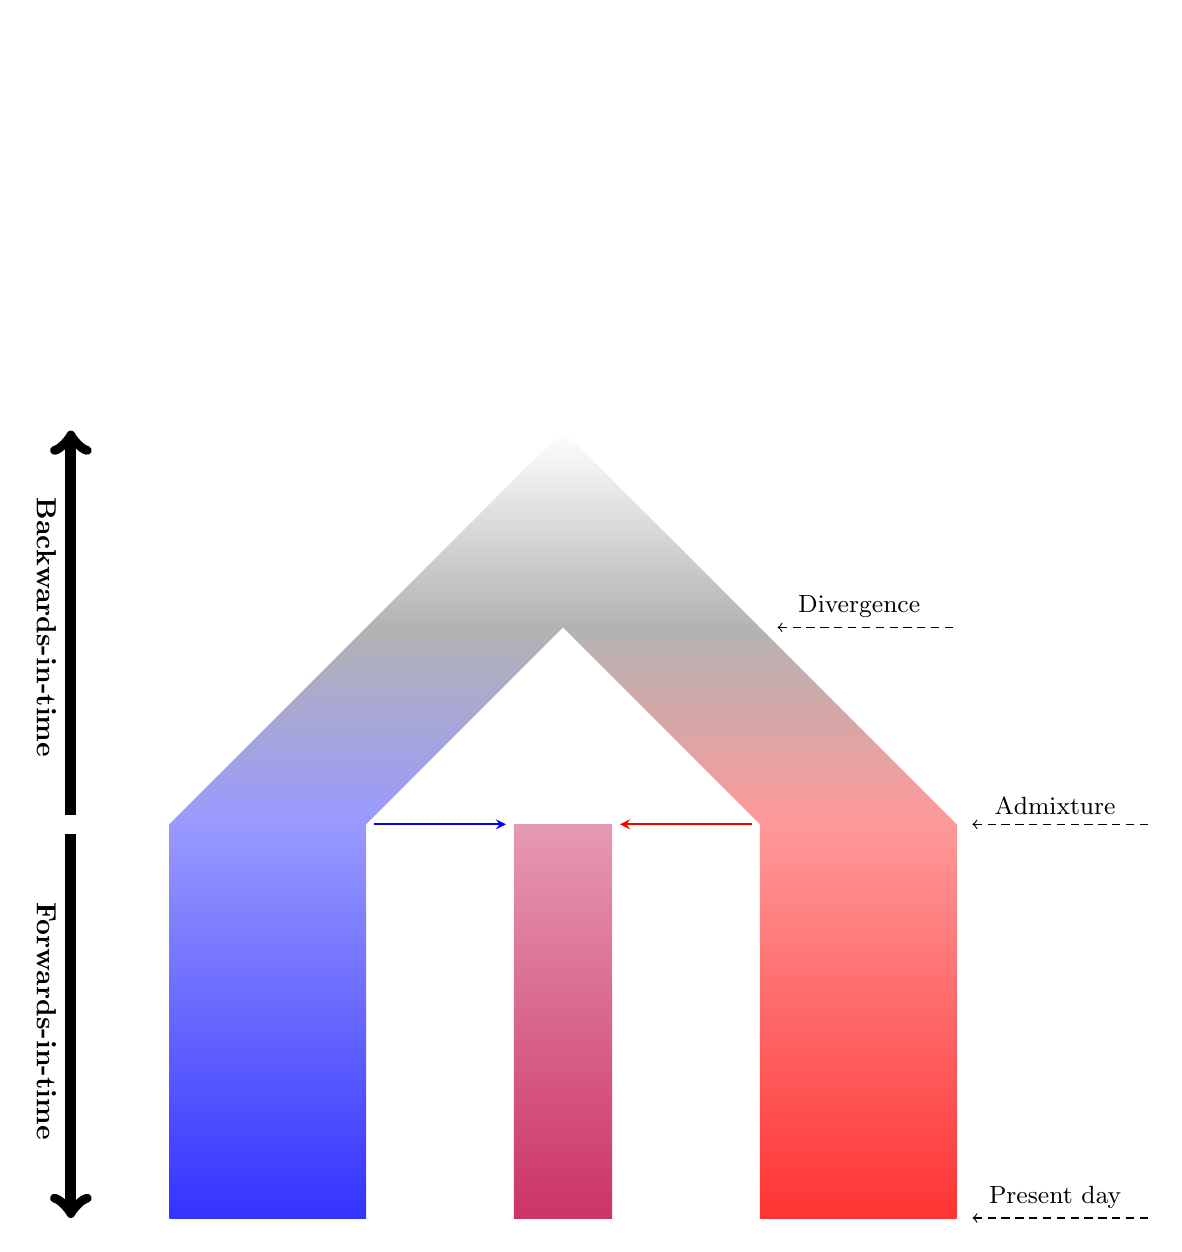
\begin{tikzpicture}[scale=.5,auto]

% Nodes
\node (mcra) at (0,0) {};
\node (admix-event) at (0,10) {};
\node (pop1) at (-10,0) {};
\node (pop2) at (10,0) {};
\node (popsize) at (5,0) {};
\node (admix-gens) at (0,10) {};
\node (split-time) at (0,5) {};
\node (adm-popsize) at ($0.5*(popsize)$) {};

% The Population tree
\node[inner sep=0] (transition1) at ($-1*(popsize) - (split-time)$) {};
\node[inner sep=0] (transition2) at ($(popsize) - (split-time)$) {};
\shade[top color=white,bottom color=black!30] (mcra.center) -- (transition1.center) -- (transition2.center) -- cycle;
\shade[top color=black!30,bottom color=blue!40] (transition1.center) -- ++(transition1.center) -- ++(popsize.center) -- ++($-1*(transition1)$) -- cycle;
\shade[top color=black!30,bottom color=red!40] (transition2.center) -- ++(transition2.center) -- ++($-1*(popsize.center)$) -- ++($-1*(transition2)$) -- cycle;
\shade[top color=blue!40,bottom color=blue!80] ($2*(transition1)$) -- ++($-1*(admix-gens)$) -- ++(popsize.center) -- ++(admix-gens.center) -- cycle;
\shade[top color=red!40,bottom color=red!80] ($2*(transition2)$) -- ++($-1*(admix-gens)$) -- ++($-1*(popsize.center)$) -- ++(admix-gens.center) -- cycle;

% The admixed population
\shade[top color=purple!40,bottom color=purple!80] ($(mcra) - 2*(split-time) - 0.5*(adm-popsize)$) -- ++(adm-popsize.center) -- ++($-1*(admix-gens)$) -- ++($-1*(adm-popsize)$) -- cycle;

% The admixture arrows
\draw[->,>=stealth,blue,semithick,shorten <=1mm,shorten >=1mm] ($-1*(split-time) + (transition1)$) -- +($0.75*(popsize)$);
\draw[->,>=stealth,red,semithick,shorten <=1mm,shorten >=1mm] ($-1*(split-time) + (transition2)$) -- +($-0.75*(popsize)$);

% The time arrows
\draw[<->,line width=4pt] ($(mcra) - 2.5*(popsize)$) -- node[below,rotate=270] {\bf Backwards-in-time} ++($-2*(split-time)$)  --  node[below,rotate=270] {\bf Forwards-in-time} ++($-2*(split-time)$) ;
\node[rectangle,fill=white] at ($(mcra) - 2.5*(popsize) - 2*(split-time)$) {};

% Time labels
\draw[<-,densely dashed,shorten <=2mm] (transition2) -- node[above] {\small Divergence}  ++(5,0);
\draw[<-,densely dashed,shorten <=2mm] ($2*(transition2)$) -- node[above] {\small Admixture}   ++(5,0);
\draw[<-,densely dashed,shorten <=2mm] ($2*(transition2) - (admix-gens)$) -- node[above] {\small Present day}   ++(5,0);

% Fill in annoying white lines
\draw[black!30] (transition1) -- (transition2);
\draw[blue!40] ($2*(transition1)$) -- +(5,0);
\draw[red!40] ($2*(transition2)$) -- +(-5,0);


\end{tikzpicture}  




\end{document}